\documentclass[12pt,utf8,notheorems,compress,t]{beamer}

\usepackage[english]{babel}

\usepackage{ragged2e}
\usepackage{mathtools}
\usepackage{xstring}

\usepackage[protrusion=true,expansion=false]{microtype}

\setlength\parskip{\medskipamount}
\setlength\parindent{0pt}

\title{Principal component analysis}
\newcommand{\bannerimage}{image-samples/00/small-reduced-001}
\author[Kleine Bayessche AG]{\vspace{-0.7em}\\\includegraphics[scale=0.8]{\bannerimage} \\[0.7em] Ingo Blechschmidt \\[-0.3em] {\scriptsize December 17th, 2014}}
\date{December 17th, 2014}

\usetheme{Warsaw}
\usecolortheme{seahorse}
%\usefonttheme{serif}
%\usepackage{mathpazo}
\usepackage{kurier}
\useinnertheme{rectangles}
\setbeamercolor{structure}{fg=purple}

% aus beamerouterthemeshadow.sty
\makeatletter
\setbeamertemplate{frametitle}
{%
  \nointerlineskip%
  \vskip-2pt%
  \hbox{\leavevmode
    \advance\beamer@leftmargin by -12bp%
    \advance\beamer@rightmargin by -12bp%
    \beamer@tempdim=\textwidth%
    \advance\beamer@tempdim by \beamer@leftmargin%
    \advance\beamer@tempdim by \beamer@rightmargin%
    \hskip-\Gm@lmargin\hbox{%
      \setbox\beamer@tempbox=\hbox{\begin{minipage}[b]{\paperwidth}%
          \vbox{}\vskip-.75ex%
          \leftskip0.3cm%
          \rightskip0.3cm plus1fil\leavevmode
          \centering%
          \insertframetitle%
          \ifx\insertframesubtitle\@empty%
            \strut\par%
          \else
            \par{\usebeamerfont*{framesubtitle}{\usebeamercolor[fg]{framesubtitle}\insertframesubtitle}\strut\par}%
          \fi%
          \nointerlineskip
          \vbox{}%
          \end{minipage}}%
      \beamer@tempdim=\ht\beamer@tempbox%
      \advance\beamer@tempdim by 2pt%
      \begin{pgfpicture}{0pt}{0pt}{\paperwidth}{\beamer@tempdim}
        \usebeamercolor{frametitle right}
        \pgfpathrectangle{\pgfpointorigin}{\pgfpoint{\paperwidth}{\beamer@tempdim}}
        \pgfusepath{clip}
        \pgftext[left,base]{\pgfuseshading{beamer@frametitleshade}}
      \end{pgfpicture}
      \hskip-\paperwidth%
      \box\beamer@tempbox%
    }%
    \hskip-\Gm@rmargin%
  }%
  \nointerlineskip
    \vskip-0.2pt
    \hbox to\textwidth{\hskip-\Gm@lmargin\hskip-\Gm@rmargin}
    \vskip-2pt
}
\makeatother

\setbeamertemplate{title page}[default][colsep=-1bp,rounded=false,shadow=false,bg=white]

\setbeamertemplate{navigation symbols}{}

\newcommand{\backupstart}{
  \newcounter{framenumberpreappendix}
  \setcounter{framenumberpreappendix}{\value{framenumber}}
}
\newcommand{\backupend}{
  \addtocounter{framenumberpreappendix}{-\value{framenumber}}
  \addtocounter{framenumber}{\value{framenumberpreappendix}} 
}

\newcommand*\oldmacro{}%
\let\oldmacro\insertshorttitle%
\renewcommand*\insertshorttitle{%
  \oldmacro\hfill\insertframenumber\,/\,\inserttotalframenumber\hfill}

\newcommand{\hil}[1]{{\usebeamercolor[fg]{item}{\textbf{#1}}}}

\newcommand{\img}[2]{\begin{center}\includegraphics[scale=#1]{#2}\end{center}}
\newcommand{\imageslide}[3]{\frame{\frametitle{#1}\img{#2}{#3}}}

\newcommand{\floatbox}[3]{%
  \raisebox{0pt}[0pt][0pt]{%
    \begin{picture}(0,0)(#1,#2)#3\end{picture}\leavevmode%
  }%
}

\newcommand{\RR}{\mathbb{R}}
\newcommand{\T}[1]{\boldsymbol{#1}}
\newcommand{\defeq}{\vcentcolon=}
\DeclareMathOperator{\trace}{tr}
\DeclareMathOperator{\rank}{rank}

\IfSubStr{\jobname}{\detokenize{nonotes}}{
  \setbeameroption{hide notes}
}{
  \setbeameroption{show notes}
}
\setbeamertemplate{note page}[plain]

\begin{document}

\newcommand{\titleanim}{
  \frame{\titlepage\transduration{1}\transfade[duration=5]}
  \addtocounter{framenumber}{-1}
}

\renewcommand{\bannerimage}{image-samples/00/small-reduced-001}\titleanim
\renewcommand{\bannerimage}{image-samples/00/small-reduced-002}\titleanim
\renewcommand{\bannerimage}{image-samples/00/small-reduced-003}\titleanim
\renewcommand{\bannerimage}{image-samples/00/small-reduced-004}\titleanim
\renewcommand{\bannerimage}{image-samples/00/small-reduced-005}\titleanim
\renewcommand{\bannerimage}{image-samples/00/small-reduced-006}\titleanim
\renewcommand{\bannerimage}{image-samples/00/small-reduced-007}\titleanim
\renewcommand{\bannerimage}{image-samples/00/small-reduced-008}\titleanim
\renewcommand{\bannerimage}{image-samples/00/small-reduced-009}\titleanim
\renewcommand{\bannerimage}{image-samples/00/small-reduced-010}\titleanim
\renewcommand{\bannerimage}{image-samples/00/small-reduced-009}\titleanim
\renewcommand{\bannerimage}{image-samples/00/small-reduced-008}\titleanim
\renewcommand{\bannerimage}{image-samples/00/small-reduced-007}\titleanim
\renewcommand{\bannerimage}{image-samples/00/small-reduced-006}\titleanim
\renewcommand{\bannerimage}{image-samples/00/small-reduced-005}\titleanim
\renewcommand{\bannerimage}{image-samples/00/small-reduced-004}\titleanim
\renewcommand{\bannerimage}{image-samples/00/small-reduced-003}\titleanim
\renewcommand{\bannerimage}{image-samples/00/small-reduced-002}\titleanim
\renewcommand{\bannerimage}{image-samples/00/small-reduced-001}\titleanim
\frame{\titlepage}

\frame{\frametitle{Outline}
  \floatbox{-200}{70}{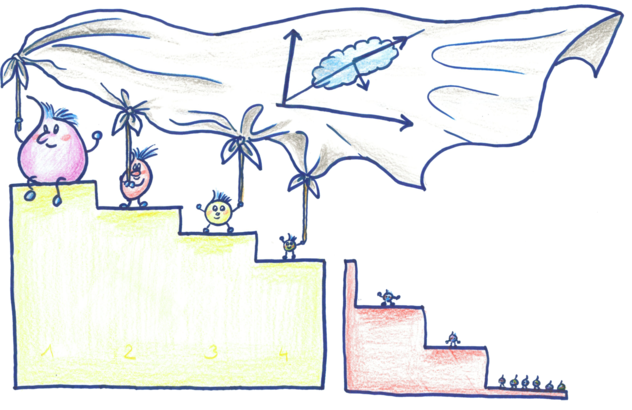
\includegraphics[width=0.4\textwidth]{svd}}
  \vspace{-1em}
  \tableofcontents
}

\section{Theory}

\subsection[SVD]{Singular value decomposition}

\frame{\frametitle{Singular value decomposition}
  Let~$A \in \RR^{n \times m}$. Then there exist
  \begin{itemize}
    \item numbers~$\sigma_1 \geq \sigma_2 \geq \cdots \geq \sigma_m \geq 0$,
    \item an orthonormal basis~$\T{v}_1,\ldots,\T{v}_m$ of~$\RR^m$, and
    \item an orthonormal basis~$\T{w}_1,\ldots,\T{w}_n$ of~$\RR^n$,
  \end{itemize}
  such that
  \begin{align*}
    A \T{v}_i &= \sigma_i \T{w}_i, \quad i = 1,\ldots,m. \\
  \intertext{In matrix language:}
    A &= W \Sigma V^t, \\
    \text{where}\quad
    V &= (\T{v}_1|\ldots|\T{v}_m) \in \RR^{m \times m}\text{ orthogonal}, \\
    W &= (\T{w}_1|\ldots|\T{w}_n) \in \RR^{n \times n}\text{ orthogonal}, \\
    \Sigma &= \mathrm{diag}(\sigma_1,\ldots,\sigma_m) \in \RR^{n \times m}.
  \end{align*}
}

\note{
  \begin{itemize}
    \justifying
    \item The singular value decomposition (SVD) exists for any real matrix,
    even rectangular ones.
    \item The singular values~$\sigma_i$ are unique.
    \item The basis vectors are not unique.
    \item If~$A$ is orthogonally diagonalizable with eigenvalues~$\lambda_i$
    (for instance, if~$A$ is symmetric), then~$\sigma_i = |\lambda_i|$.
    \item $\|A\|_\text{Frobenius} = \sqrt{\sum_{ij} A_{ij}^2} =
    \sqrt{\trace(A^tA)} = \sqrt{\sum_i \sigma_i^2}$.
    \item There exists a generalization to complex matrices. In this case, the
    matrix~$A$ can be decomposed as~$W \Sigma V^\star$, where~$V^\star$ is the
    complex conjugate of~$V^t$ and~$W$ and~$V$ are unitary matrices.
    \item The singular value decomposition can also be formulated in a
    basis-free manner as a result about linear maps between finite-dimensional
    Hilbert spaces.
  \end{itemize}
}

\note{
  Existence proof (sketch):
  \begin{enumerate}
    \justifying
    \item Consider the eigenvalue decomposition of the symmetric and
    positive-semidefinite matrix~$A^t A$: We have an orthonormal
    basis~$\T{v}_i$ of eigenvectors corresponding to eigenvalues~$\lambda_i$.
    \item Set~$\sigma_i \defeq \sqrt{\lambda_i}$.
    \item Set~$\T{w}_i \defeq \frac{1}{\sigma_i} A \T{v}_i$ (for those~$i$
    with~$\lambda_i \neq 0$).
    \item Then~$A \T{v}_i = \sigma_i \T{w}_i$ holds trivially.
    \item The~$\T{w}_i$ are orthonormal: $(\T{w}_i,\T{w}_j) = \frac{1}{\sigma_i
    \sigma_j} (A^t A \T{v}_i, \T{v}_j) = \frac{\lambda_i \delta_{ij}}{\sigma_i
    \sigma_j}$.
    \item If necessary, extend the~$\T{w}_i$ to an orthonormal basis.
  \end{enumerate}

  \justifying
  This proof gives rise to an algorithm for calculating the SVD, but
  unless~$A^t A$ is small, it has undesirable numerical properties.
  (But note that one can also use~$A A^t$!) Since the
  1960ies, there exists a stable iterative algorithm by Golub and van Loan.
  \par
}


\subsection{Pseudoinverses}

\frame{\frametitle{The pseudoinverse of a matrix}
  Let~$A \in \RR^{n \times m}$ and~$\T{b} \in \RR^n$. Then the solutions to the
  optimization problem
  \[ \|A\T{x} - \T{b}\|_2 \longrightarrow \text{min} \]
  under~$\T{x} \in \RR^m$ are given by
  \begin{align*}
    \T{x} &= A^+ \T{b} + V \begin{pmatrix}0\\\star\end{pmatrix}, \\
  \intertext{where $A = W \Sigma V^t$ is the SVD and}
    A^+ &= W \Sigma^+ V^t, \\
    \Sigma^+ &= \mathrm{diag}(\sigma_1^{-1},\ldots,\sigma_m^{-1}).
  \end{align*}
}

\note{
  \begin{itemize}
    \justifying
    \item In the formula for~$\Sigma^+$, set~$0^{-1} \defeq 0$.
    \item If~$A$ happens to be invertible, then~$A^+ = A^{-1}$.
    \item The pseudoinverse can be used for polynomial approximation:
    Let data points $(x_i,y_i) \in \mathbb{R}^2$, $1 \leq i \leq N$, be given.
    Want to find a polynomial $p(z) = \sum_{k=0}^n \alpha_i z^i$, $n \ll N$,
    such that
    \[ \sum_{i=1}^N |p(x_i) - y_i|^2 \longrightarrow \text{min.} \]
    In matrix language, this problem is written
    \[ \|A \T{u} - \T{y}\|_2 \longrightarrow \text{min} \]
    where $\T{u} = (\alpha_0,\ldots,\alpha_N)^T \in \mathbb{R}^{n + 1}$ and
    \[ A = \begin{pmatrix}
      1 & x_1 & x_1^2 & \cdots & x_1^n \\
      1 & x_2 & x_2^2 & \cdots & x_2^n \\
      \vdots & \vdots & \vdots & \ddots & \vdots \\
      1 & x_N & x_N^2 & \cdots & x_N^n
    \end{pmatrix} \in \mathbb{R}^{N \times (n+1)}, \quad
    \T{y} = \begin{pmatrix}y_1 \\ y_2 \\ \vdots \\ y_N\end{pmatrix} \in \mathbb{R}^{N}. \]
  \end{itemize}
}


\subsection{Low-rank approximation}

\frame{\frametitle{Low-rank approximation}
  Let~$A = W \Sigma V^t \in \RR^{n \times m}$ and~$1 \leq r \leq n,m$. Then a
  solution to the optimization problem
  \[ \|A - M\|_\text{Frobenius} \longrightarrow \text{min} \]
  under all matrices~$M$ with~$\rank{M} \leq r$ is given by
  \begin{align*}
    M &= W \Sigma_r V^t, \\
    \text{where}\quad
    \Sigma_r &= \mathrm{diag}(\sigma_1,\ldots,\sigma_r,0,\ldots,0).
  \end{align*}

  The approximation error is
  \[ \|A - W \Sigma_r V^t\|_\text{F} = \sqrt{\sigma_{r+1}^2 + \cdots + \sigma_m^2}. \]
}

\note{
  \begin{itemize}
    \item This is the Eckart--Young(--Mirsky) theorem.
    \item Beware of false and incomplete proofs in the literature!
  \end{itemize}
}


\section{Applications}

\subsection{Image compression}

\frame{\frametitle{Image compression}
  \begin{itemize}
    \item Think of images as matrices.
    \item Substitute a matrix~$W \Sigma V^t$ by $W \Sigma_r V^t$ with $r$
    small.
    \item To reconstruct $W \Sigma_r V^t$, only need to know
    \begin{itemize}
      \item the $r$ singular values $\sigma_1,\ldots,\sigma_r$,
      \hfill $r$
      \item the first $r$ columns of $W$, and
      \hfill $\text{height} \cdot r$
      \item the top $r$ rows of $V^t$.
      \hfill $\text{width} \cdot r$
    \end{itemize}
    \item Total amount: $r \cdot (1 + \text{height} + \text{weight}) \ll
    \text{height} \cdot \text{width}$
  \end{itemize}
}

\note{
  \begin{itemize}
    \justifying
    \item Image compression by singular value decomposition is mostly of
    academic interest only.
    \item This might be for the following reasons: other compression algorithms
    have more efficient implementations; other algorithms taylor to the
    specific properties of human vision; the basis vectors of other approaches
    (for instance, DCT) are similar to the most important singular basis
    vectors of a sufficiently large corpus of images.
  \end{itemize}
}


\subsection[POD]{Proper orthogonal decomposition}

\frame{\frametitle{Proper orthogonal decomposition}
  Given data points~$\T{x}_i \in \RR^N$, want to find a low-dimensional
  linear subspace which \hil{approximately contains} the~$\T{x}_i$.

  Minimize
  \[ J(U) \defeq \sum_i \|\T{x}_i - P_U(\T{x}_i)\|^2 \]
  under all~$r$-dimensional subspaces~$U \subseteq \RR^N$, $r \ll N$,
  where~$P_U : \RR^N \to \RR^N$ is the orthogonal projection onto~$U$.
  \pause

  More concrete formulation: Minimize
  \[ J(\T{u}_1,\ldots,\T{u}_r) \defeq
    \sum_i \Bigl\|\T{x}_i - \sum_{j=1}^r \langle\T{x}_i,\T{u}_j\rangle
    \T{u}_j\Bigr\|^2, \]
  where~$\T{u}_1,\ldots,\T{u}_r \in \RR^N$, $\langle\T{u}_j,\T{u}_k\rangle =
  \delta_{jk}$.
}

\note{
  Collect the data points~$\T{x}_i$ as columns of a matrix
  \[ X = (\T{x}_1 | \cdots | \T{x}_\ell) \in \RR^{N \times \ell} \]
  and consider its singular value decomposition
  \[ X = W \Sigma V^t. \]
  Then a solution to the minimization problem is given by the first~$r$ columns
  of~$W$, with approximation error
  \[ J = \sum_i \|\T{x}_i\|^2 - \sum_{j=1}^r \sigma_j^2. \]
}

\note{
  \begin{itemize}
    \justifying
    \item Proper orthogonal decomposition (POD) cannot be used to find
    low-dimensional \emph{submanifolds} which approximately contain given data
    points. But check out \emph{kernel principal component analysis}.
    \item Also, POD does not work well with \emph{affine} subspaces. But in
    this case, the fix is easy: Simply shift the data points so that their mean
    is zero.
    \item POD is a general method for \emph{dimension reduction} and can be
    used as a kind of ``preconditioner'' for many other algorithms: Simply
    substitute the given points~$\T{x}_i$ by their projections~$P_U(\T{x}_i)$.
    \item The optimal subspace~$U$ is, in general, not unique. The POD basis is
    never unique, since~$J$ is invariant under the action of~$O(r)$.
  \end{itemize}
}


\subsection[PCA]{Principal component analysis}

\frame{\frametitle{Principal component analysis}
  Given observations~$x_i^{(k)}$ of random variables~$X^{(k)}$, want
  to find \hil{linearly uncorrelated} principal components.

  Write $X = (\T{x}_1 | \cdots | \T{x}_\ell) \in \RR^{N \times \ell}$.
  Calculate $X = W \Sigma V^t$.
  Then the principal components are the variables
  \[ Y^{(j)} = \sum_k W_{kj} X^{(k)}. \]

  Most of the variance is captured by $Y^{(1)}$; second to most is captured by
  $Y^{(2)}$; and so on.
}

\note{
  \begin{itemize}
    \justifying
    \item For instance, in a study about circles, the variables \emph{radius},
    \emph{diameter}, and \emph{circumference} are linearly correlated.
    \item Principal component analysis (PCA) would automatically pick one of
    these attributes as a principal component.
    \item We have to normalize the data to have zero empirical mean first. Then
    $XX^t$ is the empirical covariance matrix.
    \item Note that, in the given sample, the $Y^{(j)}$ are indeed
    uncorrelated:
    \begin{align*}
      E(Y^{(j)} XX^t Y^{(k)}) &= (W \T{e}_j)^t XX^t (W \T{e}_k) \\
      &= \T{e}_j^t W^t W \Sigma V^t V \Sigma^t W^t W \T{e}_k \\
      &= \Sigma \Sigma^t.
    \end{align*}
    \item Beware that PCA cannot resolve nonlinear correlation.
    \item Also note that PCA is sensitive to outliers and not
    scaling-independent.
  \end{itemize}
}


\subsection{Eigenfaces}

\frame{\frametitle{Eigenfaces}
  \begin{columns}[T]
    \begin{column}{0.6\textwidth}
      \begin{itemize}
        \item Record sample faces $\T{x}_1,\ldots,\T{x}_N \in \RR^{\text{width}
        \cdot \text{height}}$.
        \item Calculate a POD basis of \hil{eigenfaces}.
        \item Recognize faces by looking at the coefficients of the most
        important eigenfaces.
      \end{itemize}
    \end{column}
    \begin{column}{0.4\textwidth}
      \centering
      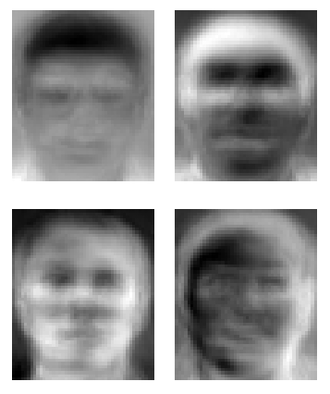
\includegraphics[width=\textwidth]{eigenfaces-1} \\
      \scriptsize
      Eigenfaces resemble faces.\par
    \end{column}
  \end{columns}
}

\imageslide{More eigenfaces}{0.5}{eigenfaces-2}

\note{
  \begin{itemize}
    \justifying
    \item A naive approach is very sensitive to lighting, scale and
    translation.
    \item But extensions are possible, for instance considering the eyes, the
    nose, and the mouth separately; this leads to eigeneyes, eigennoses, and
    eigenmouths.
    \item Image credit: \\
    \url{http://upload.wikimedia.org/wikipedia/commons/6/67/Eigenfaces.png} \\
    \url{http://www.cenparmi.concordia.ca/~jdong/eigenface.gif}
    \item Live demo: \\ \url{http://cognitrn.psych.indiana.edu/nsfgrant/FaceMachine/faceMachine.html}
    \item Examples: \\ \url{http://www.cs.princeton.edu/~cdecoro/eigenfaces/}
  \end{itemize}
}


\subsection{Digit recognition}

\frame{\frametitle{Digit recognition}
  Apply POD for dimension reduction, then use some similarity measure or
  clustering technique. Results:

  \centering
  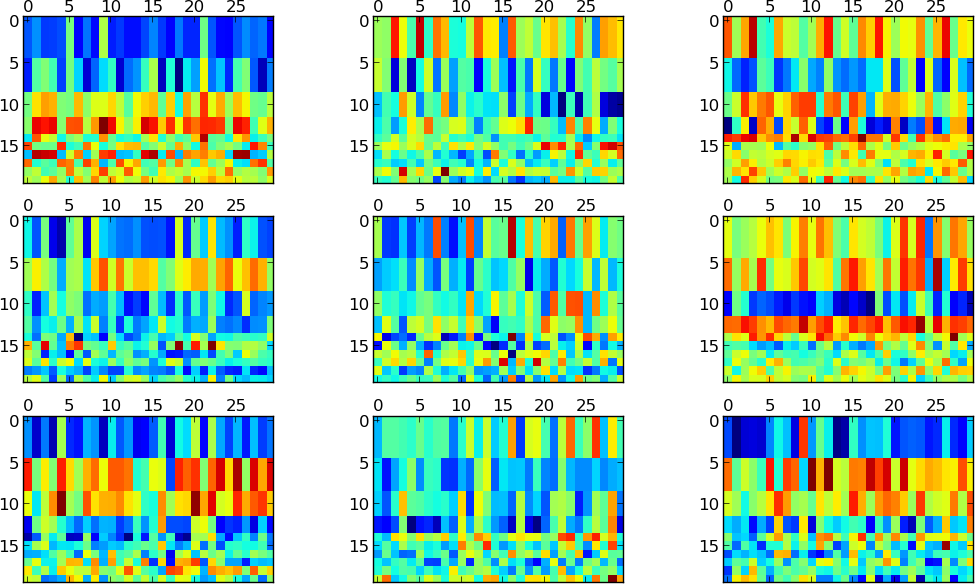
\includegraphics[width=0.95\textwidth]{pca-digit-recognition}
  \par
}

\frame{\frametitle{Eigendigits}
  \centering
  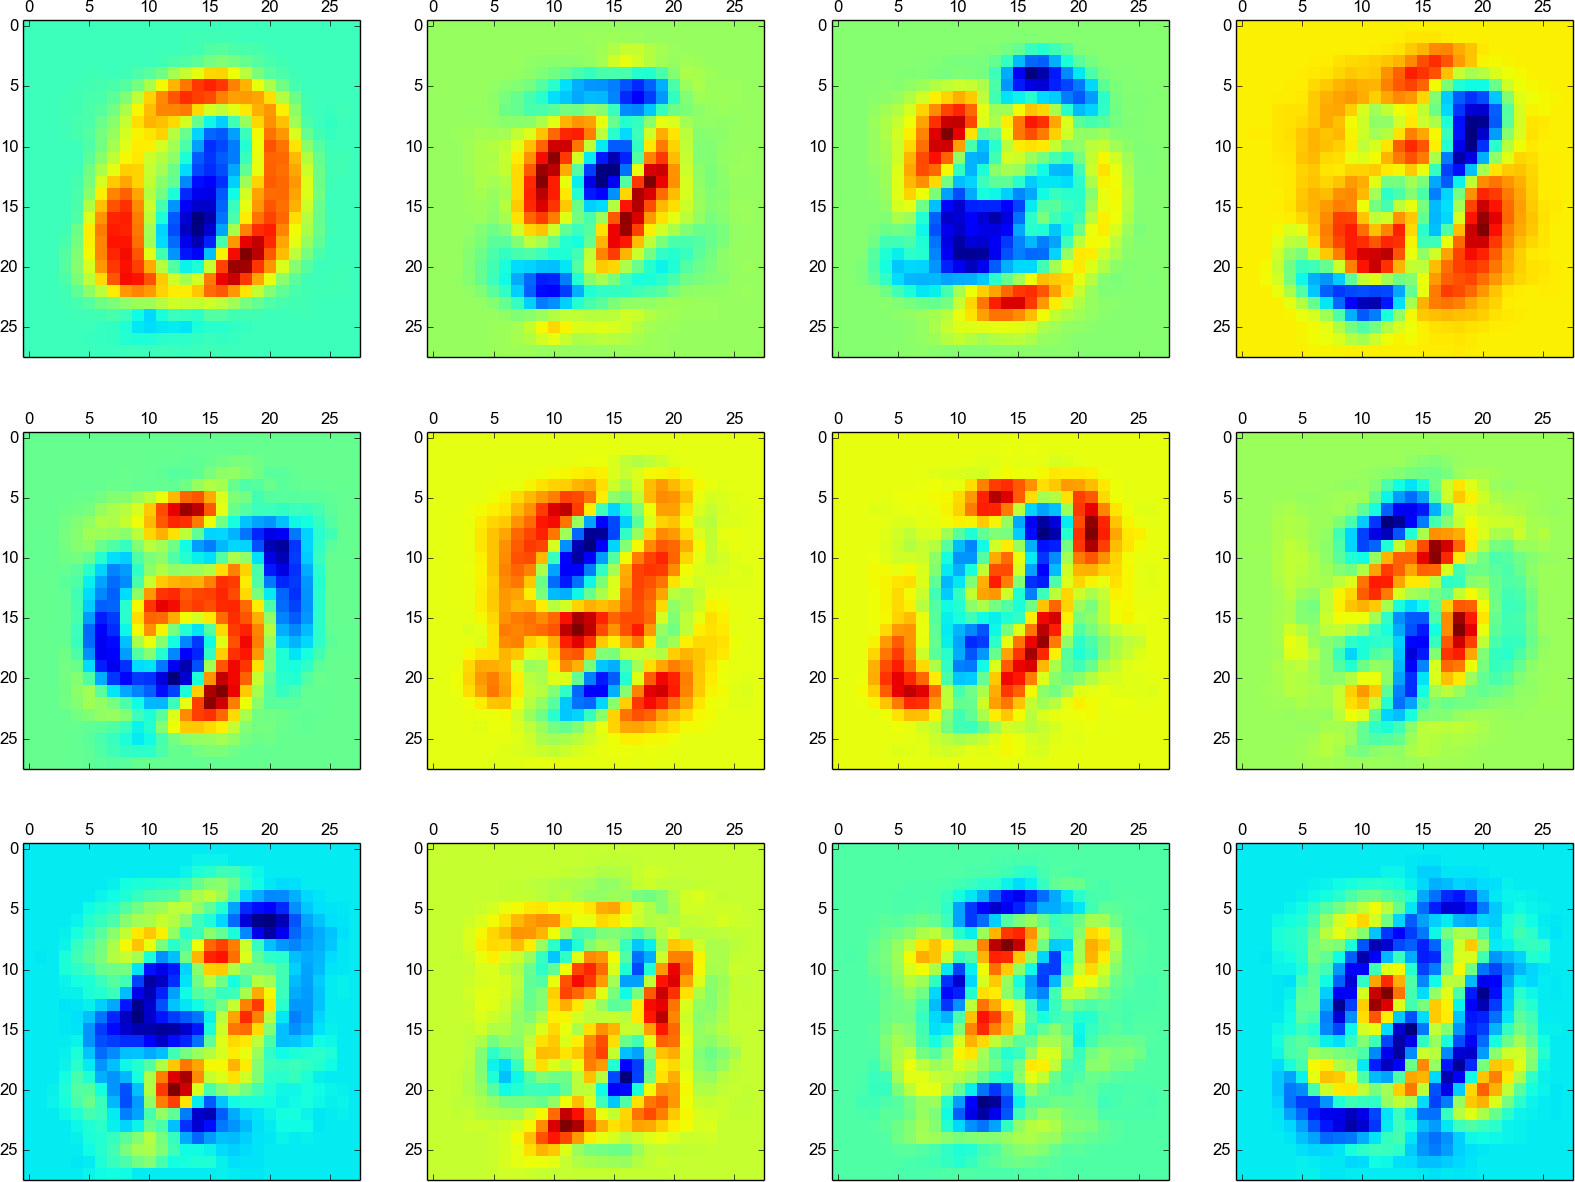
\includegraphics[width=0.95\textwidth]{eigendigits}
  \par
}

\note{
  \begin{itemize}
    \justifying
    \item This naive approach does not work very well, but refined techniques
    are discussed in the literature.
  \end{itemize}
}


\backupstart
\frame[plain]{
  \centering
  
\includegraphics[height=1.05\textheight]{i-dont-always-do-model-reduction}
  \par
}
\backupend

\end{document}

Theory
* SVD, existence and basic properties
* best-approximation in rank
* calculation
* stochastical interpretation

Applications
* POD (shortly)
* image compression
* eigenfaces
* digit recognition
* audio compression?
* Shazam?

Misc
* nonlinear generalization
* scale sensitivity
* kernel trick?

http://fc09.deviantart.net/fs70/f/2011/247/7/5/arkadia_ir_by_liquid82-d48uf64.jpg

http://upload.wikimedia.org/wikipedia/commons/3/3a/Lena_Meyer-Landrut_at_PC_after_2010_Eurovision_2.jpg
http://i.ytimg.com/vi/0YwrcZVM1MA/0.jpg
http://www.clausewitz.com/images/MandelbrotSetSM.gif
http://mathecamp.speicherleck.de/imgs/20140820_IMG_9512.jpg
http://rs2img.memecdn.com/i-dont-always-smile-but-when-i-do_o_344193.jpg
http://i.kinja-img.com/gawker-media/image/upload/s--BCSA3MoB--/18nyts1owfo9rjpg.jpg
http://static.giantbomb.com/uploads/original/1/17172/1419618-unicorn2.jpg
http://www.quickmeme.com/img/05/05e3cb3965c832e1061996f4dd3069dd69a9873937d694ea042e45232955753b.jpg
